\section{Reflection of analyticity in sumrule derivation} \label{sec:app:alyt-sr}

Amplitudes in case forward scattering are functions only of Mandelstam variable $s$, or $\nu = \frac{s - q_1^2 - q_2^2}{2}$ which makes crossing symmetry explicit. We assume, they are analytical functions of $\nu$ everywhere except real axis, where we have left- and right-hand cuts. They correspond to the threshold where new particles can be born on-shell in the photon-photon scattering. We apply Cauchy theorem with the contour shown in the figure (\cref{fig:app:sr-contour}).

\begin{figure}[H]
    \centering
    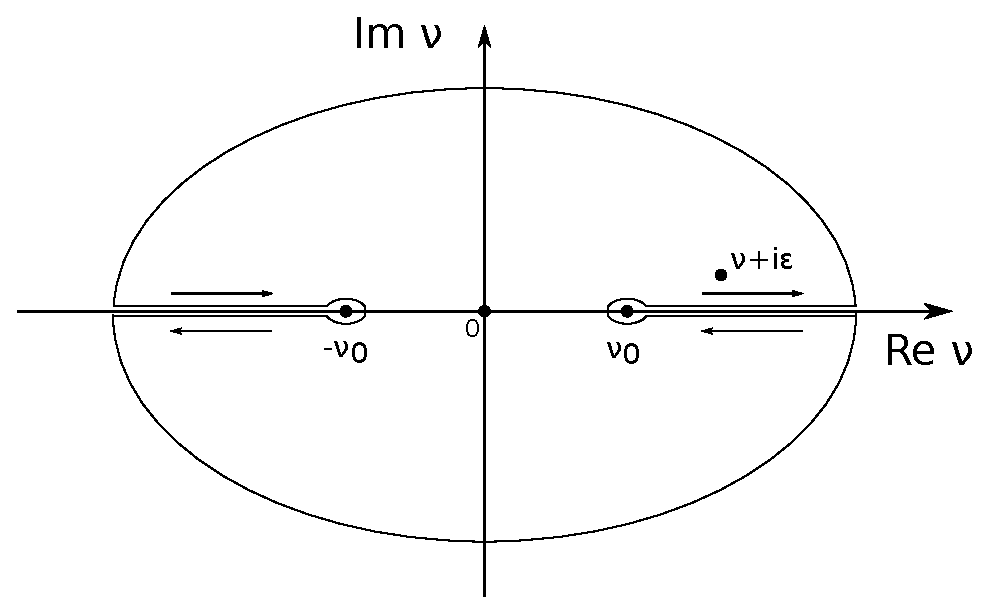
\includegraphics[width=12cm]{alyt-contour.eps}
    \caption{Integration contour in Cauchy formula used for dispersion relations. \label{fig:app:sr-contour}}
\end{figure}

According to the theorem, contour should contain $\nu$, so we shift $\nu$ into complex plane a little by setting $\nu \rightarrow \nu+\ii \delta$. Then we rewrite contour integral as a sum of integrals over simple contours. We assume integrations over infinitely distant arcs vanish as well as contributions from edges of cuts.

We denote $f^{\pm}$ even and odd amplitudes, but sometimes (in this section) we skip signs assuming they are present.

\begin{align}
    &2 \pi \ii f(\nu) = \oint \frac{f(\nu^\prime)}{\nu^\prime - \nu} \dd{\nu^\prime} \\
    \begin{split}
        &2\pi \ii f(\nu+\ii\delta) = \int_{\nu_0}^{\infty} \frac{f(\nu^\prime + \ii \epsilon)}{\nu^\prime + \ii \epsilon - \nu - \ii \delta} + \int_{\infty}^{\nu_0} \frac{f(\nu^\prime-\ii \epsilon)}{\nu^\prime - \ii \epsilon - \nu - \ii \delta} + \\
        &\quad + \int_{-\infty}^{-\nu_0} \frac{f(\nu^\prime+\ii \epsilon)}{\nu^\prime + \ii \epsilon - \nu - \ii \delta}+ \int_{-\nu_0}^{-\infty} \frac{f(\nu^\prime-\ii \epsilon)}{\nu^\prime - \ii \epsilon - \nu - \ii \delta} + \\
        &\quad + \text{vanishing contributions}
    \end{split} \label{eq:app:alyt-ampl-init}
\end{align}

We assume amplitudes are analytically continuated into complex plane with Shwartz reflection principle: $f(\nu^\star) = f^\star(\nu)$. Then crossing symmetry relation acquires the following form (we assume $\nu$ lying on the real axis):

\begin{align}
    f^{(\pm)}(-\nu+\ii \epsilon) = \pm f^{(\pm)}(\nu - \ii \epsilon) = \pm f^{(\pm)\star}(\nu + \ii \epsilon)
\end{align}

Expression for amplitude (\cref{eq:app:alyt-ampl-init}) can be simplified:
\begin{align}
    \begin{split}
        &2 \pi \ii f^{\pm}(\nu+\ii\delta) = \int_{\nu_0}^{\infty} \frac{f^{\pm}(\nu^\prime + \ii \epsilon)}{\nu^\prime + \ii \epsilon - \nu - \ii \delta} - \int_{\nu_0}^{\infty} \frac{f^{\pm}(\nu^\prime-\ii \epsilon)}{\nu^\prime - \ii \epsilon - \nu - \ii \delta} + \\
        &\quad + \int_{\nu_0}^{\infty} \frac{f^{\pm}(-\nu^\prime+\ii \epsilon)}{-\nu^\prime + \ii \epsilon - \nu - \ii \delta} - \int_{\nu_0}^{\infty} \frac{f^{\pm}(-\nu^\prime-\ii \epsilon)}{-\nu^\prime - \ii \epsilon - \nu - \ii \delta} =
    \end{split} \\
    \begin{split}
        &= \int_{\nu_0}^{\infty} \frac{f^{\pm}(\nu^\prime + \ii \epsilon)}{\nu^\prime + \ii \epsilon - \nu - \ii \delta} - \int_{\nu_0}^{\infty} \frac{f^{\pm \star}(\nu^\prime+\ii \epsilon)}{\nu^\prime - \ii \epsilon - \nu - \ii \delta} +  \\
        &\quad + \int_{\nu_0}^{\infty} \frac{\pm f^{\pm \star}(\nu^\prime+\ii \epsilon)}{-\nu^\prime + \ii \epsilon - \nu - \ii \delta} - \int_{\nu_0}^{\infty} \frac{\pm f^{\pm}(\nu^\prime+\ii \epsilon)}{-\nu^\prime - \ii \epsilon - \nu - \ii \delta}
    \end{split}
\end{align}

At this point we should neglect $\epsilon$ in comparison to $\delta$ because while $\epsilon$ represents the shore near the cut $\delta$ remains fixed shift of $\nu$.

\begin{align}
    &\pi f^{\pm}(\nu+\ii\delta) = \int_{\nu_0}^{\infty} \frac{\Im f^{\pm}(\nu^\prime + \ii \epsilon)}{\nu^\prime - (\nu+\ii \delta)} \pm \int_{\nu_0}^{\infty} \frac{\Im f^{\pm}(\nu^\prime+\ii \epsilon)}{\nu^\prime + (\nu+\ii\delta)} = \\
    &f^{+}(\nu+\ii \delta) = \frac{2}{\pi} \int_{\nu_0}^{\infty} \frac{\nu^\prime \Im f^{+}(\nu^\prime + \ii \epsilon)}{(\nu + \nu^\prime + \ii \delta)(\nu - \nu^\prime - \ii\delta)} \\
    &f^{-}(\nu+\ii \delta) = \frac{2 (\nu+\ii \delta)}{\pi} \int_{\nu_0}^{\infty} \frac{\Im f^{-}(\nu^\prime + \ii \epsilon)}{(\nu + \nu^\prime + \ii \delta)(\nu - \nu^\prime - \ii \delta)}
\end{align}

Now we apply Sokhotski-Plemelj theorem to the pole at the positive side of the real axis ($\nu^\prime = \nu+\ii \delta$), because it is only one which lies inside of the integration range.

\begin{align}
    &\int \frac{\hl{f(x^\prime)}}{x^\prime - x \pm \ii \delta} \dd{x^\prime} = \fint \frac{\hl{f(x^\prime)}}{x^\prime - x} \dd{x^\prime} \mp \ii \pi f(x) \label{app:sokh-plem} \\[1cm]
    &f^{+}(\nu+\ii \delta) = \frac{2}{\pi} \fint_{\nu_0}^{\infty} \frac{\hl{\nu^\prime Im f^{+}(\nu^\prime+\ii \epsilon)}}{\hl{(\nu^\prime + \nu + \ii \delta)}(\nu^\prime - \nu)} \dd{\nu^\prime} + \frac{2}{\pi} \frac{\hl{(\nu + \ii \delta)} \pi}{\hl{2 (\nu + \ii \delta)}} \hl{f^{-}(\nu + \ii \delta + \ii \epsilon)} \\
    &f^{-}(\nu+\ii \delta) = \frac{2 (\nu+\ii \delta)}{\pi} \fint_{\nu_0}^{\infty} \frac{\hl{Im f^{-}(\nu^\prime+\ii \epsilon)}}{\hl{(\nu^\prime + \nu + \ii \delta)}(\nu^\prime - \nu)} \dd{\nu^\prime} + \frac{2 (\nu+\ii \delta)}{\pi} \frac{\pi}{\hl{2 (\nu + \ii \delta)}} \hl{f^{-}(\nu + \ii \delta + \ii \epsilon)}
\end{align}

We highlighted objects corresponding to the function $f$ in general Sokhotski-Plemelj theorem(\cref{app:sokh-plem}). Finally: \\[1cm]

\fbox{
    \parbox{12cm}{
        \centering
        \begin{align}
            &\Re f^{+}(\nu+\ii \delta) = \frac{2}{\pi} \fint_{\nu_0}^{\infty} \frac{\nu^\prime \Im f^{-}(\nu^\prime+\ii \epsilon)}{(\nu^{\prime 2} - \nu^2)} \dd{\nu^\prime} \\
            &\Re f^{-}(\nu+\ii \delta) = \frac{2 \nu}{\pi} \fint_{\nu_0}^{\infty} \frac{\Im f^{-}(\nu^\prime+\ii \epsilon)}{(\nu^{\prime 2} - \nu^2)} \dd{\nu^\prime}
        \end{align}
    }
}
